\chapter{Separation of concerns}
Now that we got to understand the origins of cross-platform development, I believe it's time for a move that's just as important for the thesis.
During this chapter, I'll take a step towards a different direction.
I'll take a look at the definitions, because there will be multiple, history, use cases, advantages and disadvantages of the principle of separating concerns.
We'll compare and analyze the views regarding this topic, see where it originated (or all the places of its origins), 
check out what caused it to come into existence, and then do a thorough analysis regarding the benefits it provides, and the disadvantages they bring.



\section{When was introduced}
The principle of separation of concerns has roots that extend back several decades, and it has been discussed and applied in various forms across different disciplines, including software engineering, information architecture, and systems design.
While it's challenging to pinpoint an exact date or origin for this principle, we can explore some key moments in its history, the ones that got it started as a founding principle in software design.
First we'll take a look at the structured programming era, this taking place during the 1960's-1970's timeframe.
\par
During the structured programming era, pioneers such as Edsger W.
Dijkstra and Niklaus Wirth advocated for modular programming techniques that emphasized separation of concerns to improve code clarity and maintainability.
Dijkstra was the first to indirectly point towards this approach, because he argued against the unstructured use of goto statements and advocated for structured programming techniques, which inherently promote separation of concerns.
He emphasized the importance of clear control flow and modular design in creating understandable and maintainable code.
He believed that a so called "coordinate system"\cite{firstDefinitionPrinciple} can be used to describe the code in a "helpful and manageable"\cite{firstDefinitionPrinciple} manner.

\section{Rise in popularity}
The adoption of the principle of separation of concerns gained significant momentum during the late 20th century and continued into the early 21st century.
While it's challenging to pinpoint an exact time period for its increased adoption, we can identify key phases when the concept became more widely recognized and discussed:
\par
During the emergence of object-oriented programming (OOP) in the late 1970s and 1980s, the principles of modularity and separation of concerns gained prominence.
Languages like Smalltalk and Simula popularized OOP concepts such as encapsulation, inheritance, and polymorphism, which inherently promote the separation of concerns.
This period laid the groundwork for the widespread adoption of modular design principles.
\par
The 1990s saw a proliferation of publications and discussions on software design principles, design patterns, and best practices.
Influential works such as "Design Patterns: Elements of Reusable Object-Oriented Software" by the Gang of Four (Erich Gamma, Richard Helm, Ralph Johnson, John Vlissides) were published in 1994.
This book cataloged common design patterns, many of which emphasize separation of concerns.
The 1990s also witnessed the rise of agile methodologies and the growing importance of modular design in software development.
\par
In the early 2000s, there was a continued focus on modular design principles, particularly within the context of domain-driven design (DDD) and agile software development.
Eric Evans' book "Domain-Driven Design: Tackling Complexity in the Heart of Software" (2003) emphasized the importance of separating concerns within a software system to improve maintainability and alignment with business requirements.
This period saw an increasing recognition of separation of concerns as a fundamental principle in software architecture.
\par 
From the mid-2000s to the present day, separation of concerns has remained a central tenet of software engineering practices.
The advent of microservices architectures, cloud computing, and DevOps practices further underscored the importance of modular design and loose coupling.
Additionally, the proliferation of open-source software projects and collaboration platforms facilitated the exchange of knowledge and best practices related to separation of concerns.
\par
Overall, while separation of concerns has been a guiding principle in software engineering for several decades, its adoption and recognition as a fundamental design principle gained momentum during the late 20th century and continue to shape software development practices today.
The most significant publications about separation of concerns were written during the 1990s and early 2000s, coinciding with the emergence of object-oriented programming and the proliferation of design patterns and agile methodologies.


\section{Definition}
Separation of concerns is a design principle in software engineering where different parts of a system are divided to handle different responsibilities.
This makes the system easier to understand, maintain, and modify because each part focuses on a specific aspect of functionality, rather than trying to handle everything at once.
\begin{figure}[htbp]
    \centering
    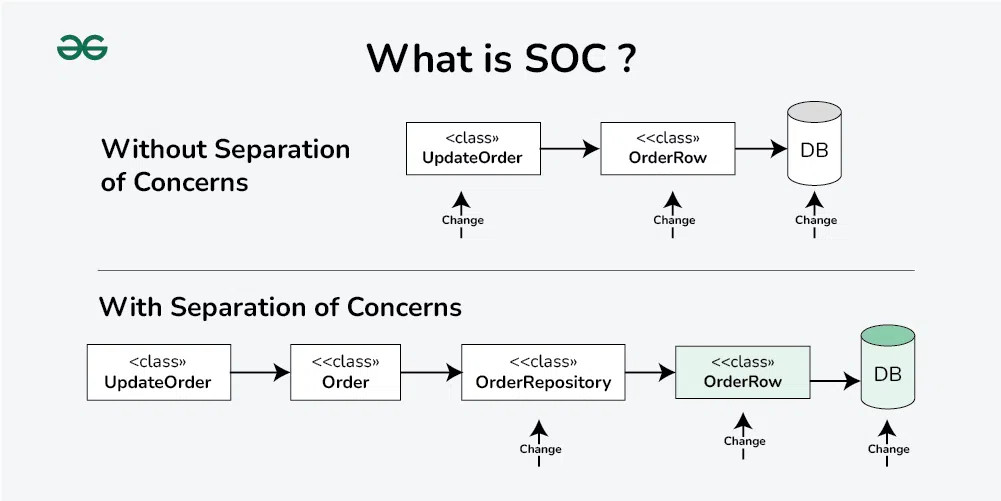
\includegraphics[scale=0.4]{pictures/soc_definition_example.jpg}
    \caption{Separation of concerns definition example, source: \href{https://www.geeksforgeeks.org/separation-of-concerns-soc/}{GeekForGeeks}}
    \label{arpanetLogicaMap}
\end{figure}
\par
Now we'll take an in-depth look at the founding ideas that are holding this principle high in its regard.
These are: modularity, flexibility and reusability, testing and scalability.
We'll take each of them apart and see what they can provide for us.


\subsection{Modularity}
Separation of concerns promotes modularity, where a system is divided into smaller, independent modules.
Each module encapsulates a specific aspect of functionality.
For example, in a web application, you might have separate modules for handling user authentication, processing data, and presenting the user interface.
\par
Modularity encourages encapsulation, which involves bundling related functionality and data into cohesive units called modules.
Each module represents a self-contained unit of code that hides its internal implementation details from the rest of the system.
This encapsulation fosters information hiding, reducing dependencies between modules and promoting loose coupling.
\par
Modular design emphasizes defining clear and well-defined interfaces for communication between modules.
These interfaces specify how modules interact with each other, providing a contract that ensures consistent behavior and interoperability.
By adhering to these interfaces, developers can swap out implementations or extend functionality without affecting other parts of the system, as long as the interface remains unchanged.
\par
Modularity allows for varying levels of granularity in module design.
Modules can be large or small, depending on the complexity and scope of the functionality they encapsulate.
Decomposing a system into smaller, more manageable modules facilitates better organization and promotes code reuse.
However, it's essential to strike a balance between granularity and cohesion to avoid overly fragmented or tightly coupled modules.
\par
Overall, modularity is a key aspect of the separation of concerns principle that promotes the organization, maintainability, and extensibility of software systems.
By breaking down a system into modular components with clear interfaces and well-defined responsibilities, developers can create more flexible, scalable, and reusable codebases.


\subsection{Readability and Maintainability}
By separating concerns, the code becomes easier to read and understand.
Developers can focus on one aspect of the system at a time, making it easier to debug, maintain, and modify without affecting other parts of the system.
This also facilitates collaboration among team members, as each person can work on different modules independently.
\par
Separation of concerns promotes clear code organization by dividing a system into distinct modules, each responsible for a specific aspect of functionality.
This modular structure makes it easier for developers to locate and understand relevant code when working on a particular feature or fixing a bug.
Clear organization reduces cognitive overload and helps developers navigate the codebase more efficiently, improving readability.
\par
By isolating concerns into separate modules, separation of concerns reduces the complexity of individual components.
Each module focuses on a specific task or responsibility, which makes the code more concise and easier to comprehend.
Developers can reason about each module in isolation, without having to consider the entire system's complexity at once, leading to improved readability.
\par
Separation of concerns aligns with the Single Responsibility Principle (SRP), which states that a module or class should have only one reason to change.
By adhering to SRP, modules become more focused and maintainable, as they are less likely to be affected by changes unrelated to their primary responsibility.
This principle enhances readability by promoting a clear understanding of each module's purpose and minimizing code churn during maintenance.
\par
Separation of concerns facilitates modular testing, where each module can be tested independently of the rest of the system.
This modular approach to testing improves maintainability by allowing developers to identify and fix bugs more efficiently.
Unit tests can be written for each module to verify its behavior in isolation, making it easier to pinpoint and resolve issues without disrupting other components.
\par
To sum it up, separation of concerns enhances readability and maintainability by promoting clear code organization, reducing complexity, adhering to the Single Responsibility Principle, isolating changes, facilitating modular testing, and encapsulating complexity.
By breaking a system into modular components with well-defined responsibilities, developers can create codebases that are easier to understand, modify, and maintain over time.


\subsection{Flexibility and Reusability} 
Separating concerns allows for greater flexibility and reusability of code.
Since each module is designed to handle a specific responsibility, it can be reused in different parts of the system or even in other projects altogether.
For example, a module responsible for database access can be reused in multiple parts of an application without modification.
\par
Separation of concerns enables a flexible system architecture by allowing each module to focus on a specific aspect of functionality.
This modular approach means that individual modules can be modified, replaced, or extended without affecting other parts of the system.
For example, if you need to change the data storage mechanism in your application, you can modify the database module without altering the modules responsible for business logic or user interface presentation.
\par
Modular design facilitates the creation of plug-and-play components that can be easily integrated into different systems or projects.
By encapsulating functionality within self-contained modules, developers can reuse these components across various applications without modification.
This promotes code reuse, accelerates development, and ensures consistency across projects.
\par
Separation of concerns encourages the creation of a library of reusable modules that can be leveraged across different projects.
These modules encapsulate common functionality, such as authentication, data validation, or file handling, making them readily available for use in new projects.
By building a library of reusable components, developers can reduce development time, minimize duplication of effort, and maintain consistency in software architectures.
\par
Separation of concerns facilitates integration with third-party libraries, frameworks, or services.
By encapsulating integration logic within modular components, developers can easily swap out implementations or upgrade dependencies without affecting the rest of the system.
This interoperability enables software systems to leverage external resources and functionalities, enhancing their capabilities and reducing development effort.
\par
When concerns are separated, changes and updates can be isolated to specific modules without affecting the rest of the system.
This isolation minimizes the risk of unintended consequences and makes it easier to test and validate modifications.
Developers can confidently refactor or extend individual modules knowing that they won't inadvertently impact other parts of the codebase, which enhances maintainability.
\par
Separation of concerns facilitates modular testing, where each module can be tested independently of the rest of the system.
This modular approach to testing improves maintainability by allowing developers to identify and fix bugs more efficiently.
Unit tests can be written for each module to verify its behavior in isolation, making it easier to pinpoint and resolve issues without disrupting other components.
\par
Modular design encapsulates complexity within well-defined boundaries, making the codebase more maintainable.
By hiding implementation details behind module interfaces, developers can interact with modules at a higher level of abstraction, reducing cognitive overhead.
This encapsulation shields developers from unnecessary complexity, enabling them to focus on understanding and maintaining one concern at a time, which enhances readability and maintainability.
\par
In summary, separation of concerns fosters flexibility and reusability by enabling modular, self-contained components that can be easily integrated, customized, extended, and reused across different projects and contexts.
This promotes agility, reduces development time, and facilitates the creation of scalable and adaptable software systems.


\subsection{Testing} 
When concerns are separated, it becomes easier to test individual modules in isolation.
This allows for more targeted and comprehensive testing, as each module can be tested independently of the rest of the system.
Additionally, modular code is often easier to mock or stub, which is useful for unit testing.
\par
Separation of concerns facilitates modular testing, where each module can be tested independently of the rest of the system.
This modular approach allows developers to write focused unit tests for individual modules, verifying their behavior in isolation.
By decoupling modules from their dependencies, such as external services or databases, developers can easily mock or stub these dependencies to create controlled test environments.
\par
When concerns are separated, testing becomes more focused and targeted.
Each module encapsulates a specific aspect of functionality, making it easier to identify and test individual behaviors.
By isolating concerns, developers can write tests that validate the correctness of each module's behavior without having to consider the interactions with other parts of the system.
This isolation simplifies testing and reduces the scope of potential failures, improving test coverage and reliability.
\par
Separation of concerns promotes clear test scenarios by defining well-defined boundaries between modules.
Each module has a clear interface and defined inputs and outputs, making it easier to identify test cases and expected outcomes.
Developers can write tests that cover various scenarios and edge cases for each module, ensuring comprehensive test coverage and robustness.
\par
Modular design enables parallel testing, where multiple modules can be tested concurrently.
Since each module operates independently of the others, developers can run tests for different modules simultaneously, reducing overall test execution time.
This parallel testing approach accelerates the feedback loop and improves the efficiency of the testing process, enabling faster iteration and delivery of software updates.
 \par
Separation of concerns enhances test maintainability by minimizing the impact of changes on test suites.
When concerns are isolated into separate modules, modifications to one module are less likely to affect the tests for other modules.
This decoupling between modules and tests reduces the need for extensive test refactoring when making changes to the codebase, ensuring that tests remain valid and reliable over time.
 \par
While separation of concerns primarily facilitates unit testing, it also supports integration testing by providing clear interfaces between modules.
Integration tests validate the interactions and collaborations between modules to ensure that they work together correctly as a cohesive system.
By testing integration points and boundary conditions, developers can identify and resolve integration issues early in the development lifecycle, improving overall system reliability.


\subsection{Scalability}
Separating concerns also facilitates scalability.
As the system grows and evolves, new functionality can be added or existing functionality can be modified without affecting other parts of the system.
This makes it easier to scale the system both horizontally (by adding more instances of existing modules) and vertically (by adding new modules).
Let's take a more in-depth look at how it influences scalability.
\par
By dividing a system into independent modules, each responsible for a specific concern, it becomes easier to manage and scale individual components.
For example, in a web application, the user interface, business logic, and data storage can be separated into distinct modules.
This isolation allows each part to be scaled independently based on demand.
Modules can be scaled according to their specific load requirements.
For instance, if the data storage module experiences heavy read/write operations, it can be scaled up by adding more database instances or using a distributed database system, without affecting the business logic or user interface modules.
\par
Separation of concerns allows for distributing the load across different modules running on separate servers or instances.
For example, microservices architecture, which heavily relies on SoC, enables distributing microservices across different nodes.
This distribution helps balance the load effectively, preventing any single component from becoming a bottleneck.
Components can be replicated across multiple servers to handle increased traffic.
For instance, multiple instances of a stateless service (e.g., an authentication service) can be run behind a load balancer to handle a larger number of requests concurrently.
\par
By isolating concerns, resources such as CPU, memory, and storage can be allocated more efficiently.
Each module can be optimized for its specific workload.
For example, a caching module can be allocated more memory, while a computation-intensive module can be allocated more CPU resources.
Cloud platforms provide features like auto-scaling, where resources are automatically added or removed based on current demand.
SoC makes it easier to apply elastic scaling to individual components, ensuring that resources are used efficiently and costs are controlled.
\par
Separation of concerns allows for optimizing the performance of individual modules without affecting the entire system.
For example, performance-critical modules such as a real-time analytics engine can be highly optimized for speed and efficiency, while less critical modules can be optimized for maintainability or other factors.
Separation of concerns facilitates the implementation of asynchronous processing.
For example, background tasks like data processing or logging can be handled by separate modules running asynchronously, reducing the load on the main application and improving overall responsiveness.
\par
When concerns are separated, updating or upgrading individual modules becomes simpler.
New features or improvements can be added to specific modules without disrupting the entire system, making it easier to evolve and scale the system over time.
Separation of concerns allows for incremental scalability, where new modules can be added to handle additional concerns as needed.
This approach ensures that the system can grow organically, adapting to new requirements and scaling efficiently.
\par
By isolating concerns, failures in one module are less likely to affect other parts of the system.
For example, if the payment processing module in an e-commerce application fails, it doesn't impact the product catalog or user authentication modules.
This isolation improves the overall resilience and scalability of the system.
In the event of partial system failures, separation of concerns allows for graceful degradation.
Non-critical modules can fail or scale down without taking down the entire system, ensuring that critical services remain operational and scalable.
\par
In summary, separation of concerns enhances scalability by enabling modular architecture, efficient resource allocation, targeted performance optimization, easier maintainability and extensibility, and improved fault isolation and recovery.
By organizing a system into distinct, manageable components, this design principle allows for focused scaling efforts, better resource utilization, and a more resilient and adaptable architecture.


\section{Challenges}
While the benefits of separating concerns are well-documented, the paradigm also introduces several challenges that developers and architects must navigate to realize its full potential.
These challenges span various aspects of software development, including design complexity, increased component management, inter-module communication, dependency management, integration testing, configuration management, and team coordination.
Understanding these challenges is crucial for effectively applying the principle and leveraging its advantages without succumbing to the pitfalls that can arise from increased system complexity.
Now we'll take a look at the mentioned challenges and analyze them.

\subsection{Complexity}
From a design perspective, separating concerns often requires designing a system with multiple modules, each responsible for a specific aspect of the functionality.
This modular design can be complex because it involves defining clear boundaries and interfaces between modules.
Ensuring that each module interacts correctly and efficiently with others can be challenging, particularly in large systems with many interdependencies.
Deciding how to partition a system into separate concerns can be non-trivial. It requires a deep understanding of the domain, potential changes, and future scalability requirements. Poorly defined boundaries can lead to tight coupling between modules, defeating the purpose of SoC.
\par
As concerns are separated, the number of components in the system increases. Managing these components, keeping track of their versions, and ensuring they are correctly integrated into the overall system can add significant complexity. Each component may have its own lifecycle, dependencies, and configuration requirements.
Deploying a system composed of many separate components can be more complex than deploying a monolithic system. Each component might need to be deployed independently, and the interactions between them must be carefully managed to ensure the system functions correctly as a whole.
\par
When enforcing the principle, different concerns are handled by different modules, which need to communicate effectively. Managing this communication can be complex, especially when different modules are developed by different teams or even at different times. Choosing the right communication protocols and ensuring data consistency across modules are critical challenges.
In a distributed system, maintaining synchronization between different modules can be difficult. Issues like data consistency, latency, and failure handling become more prominent as the number of communicating modules increases.
\par
While it aims to reduce dependencies between modules, some level of interdependency is inevitable. Managing these dependencies and ensuring that changes in one module do not adversely affect others can be complex. Dependency injection and service discovery mechanisms can help but add another layer of complexity to the system.
Keeping track of different versions of modules and ensuring compatibility between them can be challenging. This is particularly true in environments where modules are developed and released independently.
In summary, to address complexity issues, we need to keep in mind an overhead of design and architectural challenges, managing an increased number of components, ensuring effective communication and synchronization between modules, handling dependencies and versioning, and managing configurations. Addressing these challenges requires careful planning, robust tooling, and effective communication among development teams.

\subsection{Performance}
When a system is divided into separate modules, these modules often need to communicate with each other. This communication, whether it’s through function calls, message passing, or network requests, introduces latency. For instance, in a microservices architecture, each service call over the network adds a delay, which can accumulate and degrade overall system performance.
Data exchanged between modules often needs to be serialized and deserialized, especially in distributed systems. This process can be computationally expensive and add to the latency, particularly when dealing with large volumes of data or complex data structures.
\par
In systems where concurrency is heavily used, such as those employing multiple threads or asynchronous processing, the operating system may need to perform frequent context switches. This switching incurs overhead, as the CPU must save and restore the state of threads or processes, potentially leading to reduced performance.
Separate modules may require their own resources, such as memory and CPU cycles. Inefficient use of these resources across modules can lead to increased computational overhead. For example, if each module maintains its own data cache, it can lead to duplicated data and higher memory usage.
\par
In distributed systems where modules communicate over a network, the amount of data transferred between modules can become significant. High network traffic can saturate the network bandwidth, reducing throughput and affecting the performance of other network-dependent operations.
If a particular module becomes a communication bottleneck, it can slow down the entire system. For instance, a centralized database or a service handling authentication might become a performance bottleneck if it cannot handle the volume of requests efficiently.
\par
Optimizing the performance of a system with separated concerns requires comprehensive profiling and monitoring across all modules. This can be complex and resource-intensive. Identifying performance bottlenecks necessitates detailed insights into the interactions and performance metrics of each module.
Performance optimization often requires coordinated changes across multiple modules. For instance, optimizing a data processing pipeline might involve adjustments in both the data ingestion module and the processing module. Ensuring that these optimizations are harmonized can be challenging.
\par
In summary, performance challenges  need careful management, and by understanding and addressing these challenges, developers can create systems that leverage the advantages of separating concerns without compromising on performance.

\subsection{Learning curve}
Applying the principle in software development introduces a learning curve that can be challenging for developers, particularly those new to the paradigm or working within complex systems. Now, let's do an in-depth analysis at the specific learning curve challenges.
\par
Separation of concerns requires developers to think differently about how they design and structure their code. Instead of creating monolithic applications, they must learn to break down functionality into distinct, loosely-coupled modules. This shift in thinking can be difficult, especially for those accustomed to traditional, tightly-coupled designs.
Effective application of the principle demands a solid grasp of software architecture principles, including how to define clear interfaces, manage dependencies, and ensure proper module interactions. Developing these skills takes time and experience.
\par
Setting up a project while keeping the principle in mind involves creating and configuring multiple modules from the outset. This can be more complex and time-consuming than starting with a monolithic approach, requiring a good understanding of project organization and configuration management.
Developers need to familiarize themselves with tools and frameworks that also encourage the use of the principle. For instance, in a microservices architecture, knowledge of containerization (e.g., Docker), orchestration (e.g., Kubernetes), and service discovery tools becomes essential. The learning curve for these technologies can be steep.
\par
The principle often relies on well-established design patterns (e.g., Observer, Strategy, Factory, MVC, the last one being later used in a demonstrated implementation). Developers need to learn these patterns and understand when and how to apply them effectively. This involves both theoretical knowledge and practical experience.
Beyond design patterns, developers must also familiarize themselves with best practices for implementing SoC, such as encapsulation, loose coupling, and high cohesion. These principles are essential for creating maintainable and scalable systems.
\par
In summary, by providing the necessary training, tools, and support, developers overcome these challenges and effectively apply the principle to create maintainable, scalable, and high-performing systems.

\subsection{Tooling}
Implementing the separation of concerns principle in software development often necessitates the use of specialized tools to manage the increased complexity of modular systems. While these tools can greatly enhance the development process, they also introduce several challenges. Now we'll dive deeper and look at the tooling challenges associated with the principle.
\par
There is a vast array of tools available for different aspects of software development, such as version control, build automation, testing, deployment, and monitoring. Selecting the right combination of tools that work well together and support that support the principle can be daunting.
Once chosen, integrating these tools into a cohesive development environment can be challenging. Ensuring that the tools communicate effectively and that workflows are streamlined requires careful planning and configuration. Integration issues can lead to inefficiencies and disruptions in the development process.
\par
Setting up the development environment to support separation of concerns typically involves configuring multiple tools and ensuring they are correctly set up for different modules. This setup can be time-consuming and complex, especially for large projects.
Ensuring that all developers have consistent environments can be difficult. Discrepancies in tool versions, configurations, or dependencies can lead to “it works on my machine” issues, where code behaves differently on different setups.
\par
In summary, by selecting the right tools, providing comprehensive training and documentation, automating setup processes, maintaining tools regularly, streamlining debugging, and planning for scalability, organizations can effectively mitigate these challenges and leverage the full benefits of this principle.


\subsection{Debugging}
Applying the separation of concerns principle introduces several debugging challenges due to the modular and often distributed nature of the system. Let's take a look at these challenges.
\par
In a system where concerns are separated into distinct modules or services, identifying the source of an issue can be challenging. A bug in one module might manifest as an error in another, leading to confusion about where the problem actually lies.
Debugging issues that span multiple modules requires understanding the interactions and dependencies between them. This complexity increases with the number of modules and their interconnections.
\par
Each module might have its own logging mechanism, making it difficult to trace the flow of events across the entire system. Consolidating logs from different modules into a centralized logging system is essential but can be complex to set up and maintain.
Maintaining context (such as transaction IDs or user session information) across module boundaries is crucial for effective tracing. Ensuring this context is consistently propagated throughout the system can be challenging.
\par
Reproducing issues in a modular system can be difficult due to differences in development, testing, and production environments. Ensuring consistency across these environments is key but can be resource-intensive.
Each module may manage its own state, making it harder to reproduce issues that depend on specific states across multiple modules. Capturing and restoring these states for debugging purposes adds complexity.
\par
Different modules might have different error handling strategies, leading to inconsistencies in how errors are reported and propagated. Ensuring a unified error handling approach across modules is essential for effective debugging.
Debugging asynchronous operations, such as those involving message queues or background processing, adds another layer of complexity. Tracing the lifecycle of an asynchronous task across modules requires specialized tools and techniques.
\par
In summary, by employing centralized logging, distributed tracing, consistent environments, effective state management, integrated debugging tools, performance considerations, and standardized error handling, developers can mitigate these challenges and enhance their ability to debug complex modular systems effectively.

\label{chap:ch3}
